\section{Unconstrained Programming Exercices}

\subsection{Problem 1}

Discutez, suivant les valeurs du paramètre $\beta \in \mathrm{R}$, la nature des points stationnaires de la fonction de deux variables
\[
f(x,y) = x^2 + y^2 + \beta xy + x + 2y
\]

\textbf{Answer}
\begin{align*}
\nabla f(x,y) &= 
	\begin{bmatrix}
		2x + \beta y + 1 \\
		2y + \beta x + 2
	\end{bmatrix} \\
\textbf{H}(f(x,y)) &=
	\begin{bmatrix}
		2 & \beta \\
		\beta & 2
	\end{bmatrix}
\end{align*}
Find the eigen values
\begin{align*}
\text{det}(\lambda I - \textbf{H}) &= 0 \\
\text{det}\Bigg( 
	\begin{bmatrix}
		\lambda -2 & -\beta \\
		-\beta & \lambda - 2
	\end{bmatrix}
\Bigg) &= 0 \\
(\lambda -2)^2 - \beta^2 &= 0 \\
\lambda^2 -4\lambda + y - \beta^2 &= 0
\end{align*}
Using the quadratic formula
\begin{align*}
\lambda &= \frac{4 \pm \sqrt{16 - 4 \cdot 1 \cdot (4-\beta^2)}}{2} \\
&= \frac{4 \pm \sqrt{4 \beta^2}}{2} \\
&= \frac{4 \pm 2\beta}{2} \\
&= 2 \pm \beta
\end{align*}

\begin{center}
\begin{tabular}{|c|c|c|}
	\hline
	$\beta < -2$ & $\beta \in [-2, 2]$ & $\beta > 2$ \\
	\hline
	$\lambda_1 < 0$, $\lambda_2 > 0$ & $\lambda_1 = [0, 4]$, $\lambda_2 = [4, 0]$& $\lambda_1 > 0$, $\lambda_2 < 0$\\
	Indefinite matrix & Semi-definite positive matrix & Indefinite matrix\\
	\hline
	Saddle point & local minimum & saddle point \\
	\hline
\end{tabular}
\end{center}

\pagebreak
\subsection{Problem 2}

Soit la minimisation sans contraintes de la fonction
\[
f(x_1,x_2) = 2x_1^2 + x_2^2 -2x_1x_2 + 2x_1^3 + x_1^4
\]
\begin{enumerate}[(a)]
\item Trouvez les candidats solution du problème et pour chacun d’entre eux, précisez s’il s’agit d’un minimum local, d’un maximum local ou d’un point selle. Justifiez vos réponses.
\item Y a-t-il un minimum global dans ce cas? Si oui, lequel?
\end{enumerate}

\textbf{Answer}

\textbf{a)}
\begin{align*}
\nabla f(x_1, x_2) =
\begin{bmatrix}
4x_1 - 2x_2 + 6x_1^2 + 4x_1^3 \\
2x_2 - 2x_1
\end{bmatrix} &= 0\\
2x_2 - 2x_1 &\Rightarrow x_2 = x_1
\end{align*}
Substituting into the first line we get
\begin{align*}
	4x_1^3 + 6x_1^2 + 2x_1 &= 0 \\
	2x_1^3 + 3x_1^2 + x_1 &= 0 \\
	x_1(2x_1+1)(x_1+1) &=0 \\
	x_1 = 0, -1 \text{ or } -\frac{1}{2}
\end{align*}
Our 3 stationary points are $(0,0)$, $(-1,-1)$ and $(-\frac{1}{2}, -\frac{1}{2})$
\begin{align*}
\textbf{H} = 
\begin{bmatrix}
	12x_1^2 + 12x_1 + 4 & -2 \\
	-2 & 2
\end{bmatrix}
\end{align*}
Find the eigen values of the hessian
\begin{align*}
\text{det}(\lambda I - \textbf{H}) &= 0 \\
\text{det}\Bigg( 
\begin{bmatrix}
	\lambda -4(3x_1^2 + 3 x_1 + 1) & -2 \\
	-2 & \lambda -2
\end{bmatrix}
\Bigg) &= 0 \\
\Big(\lambda -4(3x_1^2 + 3 x_1 + 1)\Big)(\lambda -2) -4 &= 0
\end{align*}
For $(x_1, x_2) = (0,0)$ we have
\begin{align*}
	(\lambda-4(0-0+1))(\lambda -2 ) -4 &= 0 \\
	(\lambda -4)(\lambda -2) -4 &= 0 \\
	\lambda^2 - 6\lambda + 4 &= 0 \\
	\lambda &= \frac{6 \pm \sqrt{36 - 4 \cdot 4}}{2} \\
	\lambda &= 3 \pm \sqrt{5} \\
	\lambda_1 > 0, \lambda_2 >0
\end{align*}
Both values of $\lambda$ are positive making the Hessian definite positive at $(0,0)$ making the point a local minimum.

For $(x_1, x_2) = (1,1)$ we have
\begin{align*}
(\lambda-4(3-3+1))(\lambda -2 ) -4 &= 0 \\
(\lambda -4)(\lambda -2) -4 &= 0
\end{align*}
Which goes back to the same answer as above, thus $(1,1)$ is also a local minimum.

For $(x_1, x_2) = (-\frac{1}{2},-\frac{1}{2})$ we have
\begin{align*}
(\lambda-4(-\frac{3}{4} - \frac{6}{4} + \frac{4}{4}))(\lambda -2 ) -4 &= 0 \\
(\lambda +5)(\lambda -2) -4 &= 0 \\
\lambda^2 + 3 \lambda -14 &= 0 \\
\lambda &= \frac{-3 \pm \sqrt{9-4 \cdot 1 \cdot -14}}{2} \\
\lambda &= \frac{-3 \pm \sqrt{65}}{2}
\lambda &= 2.5311, -5.5311
\end{align*}
Meaning the Hessian is indefinite at $(-\frac{1}{2},-\frac{1}{2})$ making it a saddle point.

\subsection{Problem 3}

On dit qu’un ensemble $C \subseteq \mathrm{R}^n$ est convexe si
\[
	\lambda x+(1-\lambda )y \in C\ \ \ \forall \lambda \in [0,1],\ x, y \in C
\]

\textbf{a)} Donnez une interprétation géométrique de cette propriété et tracez un sous-ensemble de $\mathrm{R}^2$ qui n’est pas convexe.

\answer

We have two points $x$ and $y$ in $C$. If we draw a line from $x$ to $y$, the entire line has to always stay in $C$.
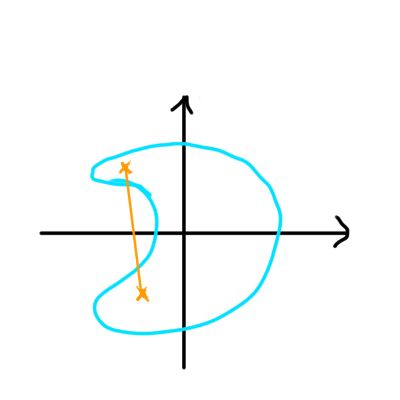
\includegraphics[scale=0.5]{fig/unconstrained_exercices/pb3a.jpg}

\pagebreak
\textbf{b)} 

\answer\footnote{\url{http://ljk.imag.fr/membres/Anatoli.Iouditski/cours/convex/chapitre_3.pdf} page 57}

Let $x,\ y\ \in C_\alpha$, take $f$ of the convex equation
\begin{align*}
f\Big(\lambda x + (1-\lambda)y \Big) &\geq f(\lambda x) + f\Big((1-\lambda)y\Big)
\intertext{Since $f$ is convex we can write by definition that}
f(\lambda x + (1-\lambda)y) &\geq f(\lambda x) + f((1-\lambda)y) \geq \lambda f(x) + (1-\lambda)f(y)
\end{align*}
Since  $x,\ y\ \in C_\alpha$ we can write
\[
f(\lambda x + (1-\lambda)y) \geq \lambda \alpha + (1-\lambda) \alpha
\]
Which is the same as
\[
f(\lambda x + (1-\lambda)y) \geq \alpha
\]
Thus $C_\alpha$ is convex
\textbf{c)}

\answer

The epigraph is the volume on top of a curve, including the curve itself. So we choose two points $(x_1, t_1)$ and $(x_2, t_2)$ both $\in \text{epi}(f)$ meaning that
\begin{align*}
	f(x_1) &\leq t_1 \\
	f(x_2) &\leq t_2
\end{align*}
To show that epi$(f)$ is convex we need to show that
\[
\lambda(x_1, t_1) + (1-\lambda)(x_2,t_2) \in \text{epi}(f)
\]
We can rewrite the lhs as the point
\[
\Big(\lambda x_1 + (1-\lambda) x_2,\ \lambda t_1 + (1-\lambda) t_2\Big) \in \text{epi}(f)
\]
which would mean that the value of $f$ from $x_1$ to $x_2$ should be less than the line $t_1$ to $t_2$ for any $\lambda \in [0, 1]$ i.e.
\[
f(\lambda x_1 + (1-\lambda) x_2) \overset{?}{\leq} \lambda t_1 + (1-\lambda) t_2
\]
Since $f$ is convex we can write
\[
f(\lambda x_1 + (1-\lambda) x_2) \leq\ \lambda f(x_1) + (1-\lambda)f(x_2) \ \leq \lambda t_1 + (1-\lambda) t_2
\]
which means the previous equation is true, thus epi$(f)$ is convex.

\textbf{d)}

\answer

We want to show that for two points $x_1,\ x_2 \in M$ we have
\[
\lambda x_1 + (1-\lambda)x_2 \in M
\]
We can do this by showing that the linear combination of $x_1$ and $x_2$ is still a minimum of $f$.
\[
f(\lambda x_1 + (1-\lambda)x_2) \overset{?}{\leq} f(x)\ \ \ \ \forall x
\]
Since $f$ is convex we can write
\[
\lambda f(x_1) + (1-\lambda)f(x_2) \overset{?}{\leq} f(x)
\]
But since $x_1$ and $x_2$ are both global minima of $f$ then $f(x_1) = f(x_2)$ and we can write
\begin{align*}
\big(\lambda + (1-\lambda)\big)f(x_1) &\overset{?}{\leq} f(x) \\
f(x_1) &\overset{?}{\leq} f(x)
\end{align*}
Which is true since we know $x_1$ is a global minimum. Thus the set $M$ is convex.

\textbf{e)}

\answer
\begin{center}
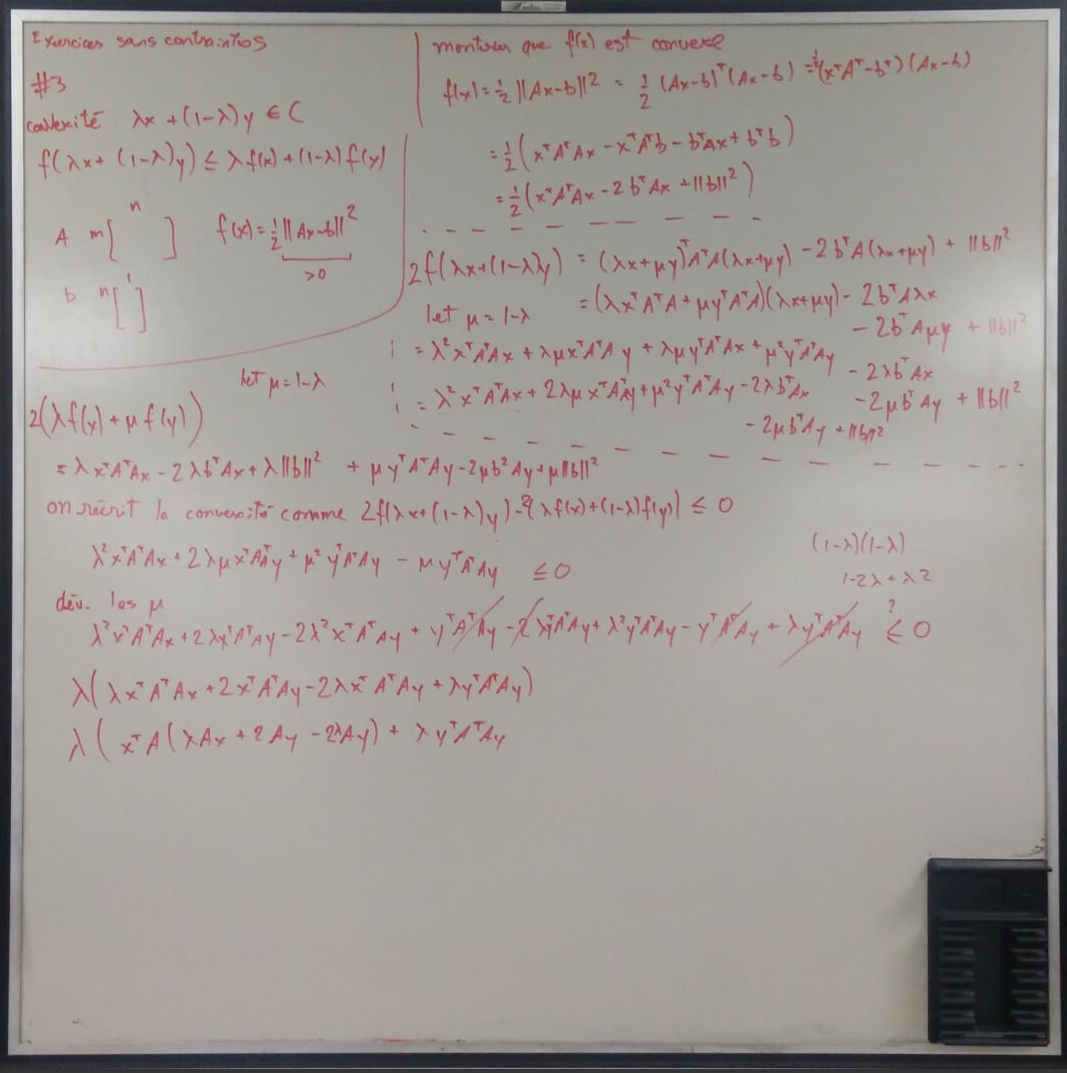
\includegraphics[width=0.75\linewidth]{fig/unconstrained_exercices/pb3_e.png}
\end{center}

Terms are supposed to cancel out... 

\incomplete

\subsection{Problem 4}

\textbf{a)}

\answer

Go back to the taylor expansion where
\[
	f(x+h) = f(x) + \nabla f(x)^Th + \text{o}(\| h\|)
\]

So we apply this to $f(x)$ which gives

\begin{align*}
	\frac{1}{2} \| F(x+h) \|^2 &= \frac{1}{2} \| F(x) + \nabla F(x)^Th + \text{o}(\| h\|) \|^2 \\
\intertext{Recall the identity $\| a + b + c\|^2 = \|a\| + \|b\| + \|c\| + 2<a,b> + 2<a,c> + 2<b,c>$}
	&= \frac{1}{2} \|  F(x)\|^2 \textcolor{red}{+ \frac{1}{2} \|  \nabla F(x)^Th\|^2}
		+ F(x)^T \nabla F(x)^Th \textcolor{red}{+ F(x)o(\|h\|) + \nabla F(x)^ThF(x)o(\|h\|)}
\end{align*}

All the red terms above are basically the error term of the Taylor expansion. By inspection we can then see that 
\begin{align*}
	\nabla f(x)^T &= F(x)^T\nabla F(x)^T \\
	\nabla f(x) &= F(x) \nabla F(x)
\end{align*}


Where if we supopose $F: \mathbb{R}^n \rightarrow \mathbb{R}^n$ then

\[
F(x_1, \ldots, x_n) =
\begin{bmatrix}
	F_1(x_1, \ldots, x_n) \\
	\vdots \\
	F_n(x_1, \ldots, x_n)
\end{bmatrix}
\]

and

\[
\nabla F(x) =
\begin{bmatrix}
	\frac{\partial F_1}{\partial x_1} & \frac{\partial F_2}{\partial x_1} & \ldots & \frac{\partial F_n}{\partial x_1} \\
	\frac{\partial F_1}{\partial x_2} & \\
	\vdots \\
	\frac{\partial F_1}{\partial x_n} & \ldots & & \frac{\partial F_n}{\partial x_n}
\end{bmatrix}
\]


\textbf{b)}

Since the gradient above is shown to be 2D we need to add a third dimension a \textcolor{red}{?tensor?} to describe the Hessian. So we have something like

\[
\nabla^2 F(x) =
\begin{bmatrix}
\frac{\partial F_1}{\partial x_1 x_1} & \frac{\partial F_1}{\partial x_1 x_2} & \ldots & \frac{\partial F_1}{\partial x_1 x_n} \\
\frac{\partial F_1}{\partial x_2 x_1} & \\
\vdots \\
\frac{\partial F_1}{\partial x_n x_1} & \ldots & & \frac{\partial F_1}{\partial x_n x_n}
\end{bmatrix},
\begin{bmatrix}
\frac{\partial F_2}{\partial x_1 x_1} & \frac{\partial F_2}{\partial x_1 x_2} & \ldots & \frac{\partial F_2}{\partial x_1 x_n} \\
\frac{\partial F_2}{\partial x_2 x_1} & \\
\vdots \\
\frac{\partial F_2}{\partial x_n x_1} & \ldots & & \frac{\partial F_2}{\partial x_n x_n}
\end{bmatrix},\ \ldots,\
\begin{bmatrix}
\frac{\partial F_n}{\partial x_1 x_1} & \frac{\partial F_n}{\partial x_1 x_2} & \ldots & \frac{\partial F_n}{\partial x_1 x_n} \\
\frac{\partial F_n}{\partial x_2 x_1} & \\
\vdots \\
\frac{\partial F_n}{\partial x_n x_1} & \ldots & & \frac{\partial F_n}{\partial x_n x_n}
\end{bmatrix}
\]

Which allows us to describe the Hessian of $f(x)$  as
\begin{align*}
\nabla^2 f(x) &= (F(x) \nabla F(x))' \\
&= \nabla F(x) \nabla F(x) + F(x) \nabla^2 F(x)
\end{align*}

Which then allos us to say that the descent direction $d$ is
\begin{align*}
	d &= - (\nabla^2 f(x))^{-1} \nabla f(x) \\
	  &= - \Bigg(\nabla F(x) \nabla F(x) + F(x) \nabla^2 F(x) \Bigg)^{-1} F(x) \nabla F(x)
\end{align*}


\textbf{c)}

\incomplete

\subsection{Problem 5}

\[
f(x_1, x_2) = 2x_1^2 -2x_1x_2 + x_2^2 + 2x_1 -2x_2
\]

Apply the steepest descent method with no linesearch starting at $(x_1, x_2) = (0,0)$

\answer

Find the gradient

\[
	\nabla f(x_1, x_2) = 
	\begin{bmatrix}
		4x_1 - 2x_2 + 2 \\
		-2x_1 + 2x_2 - 1	
	\end{bmatrix}
\]

\begin{enumerate}
\item $x_0 = (0,0)$, $k = 0$
\item $d_0 = - \nabla f((0,0)) = - \begin{bmatrix}
2 \\
1
\end{bmatrix}$
\item $x_1 = x_0 + d_k$ \\
$x_1 = \begin{bmatrix}
0 \\ 0
\end{bmatrix} - \begin{bmatrix}
2 \\ 1
\end{bmatrix} = (-2,\ -1)$
\end{enumerate}

Since there is a minimum at $(0,\ 1)$ it is clear that we went in the wrong direction. It is also clear that we went that way by a lot, so this method might never converge.

\subsection{Problem 6}

\incomplete

\subsection{Problem 7}

\textbf{a)}

\begin{lstlisting}[style=Matlab-editor]
function [f, g, H] = obj1(point)
% obj1 First objective function
% f_1(x,y_ = 2x^3 - 3x^2 -6xy(x-y-1)
% Inputs
%   x   Point at which to evaluate the function
% Output
%   f   Result of the function evaluated at x
%   g   Result of the gradient evaluated at x
%   H   Result of the Hessian evaluated at x

x = point(1);
y = point(2);

% function
f = 2*x^3 - 3*x^2 - 6*x*y*(x-y-1);

% gradient
g = [   6 * (x^2 -x -2*x*y +y^2 +y);
        6*x*(2*y - x + 1)];

% hessian
H = [   12*x-12*y-6,        12*y - 12*x + 6; ...
        12*y - 12*x + 6,    12*x];

\end{lstlisting}


\begin{lstlisting}[style=Matlab-editor]
function [f, g, H] = obj2(x)
% obj2 Second objective function if problem 7
%   
% Inputs
%   x   Point at which to evaluate the function
% Output 
%   f   Result of the function evaluated at x
%   g   Result of the gradient evaluated at x
%   H   Result of the Hessian evaluated at x
% Author: Andre Phu-Van Nguyen <andre-phu-van.nguyen@polymtl.ca>

f = 0;
n = length(x) - 1;
for i = 1:n
    tmp = 100 * (x(i+1) - x(i)^2)^2 + (1-x(i))^2;
    f = f + tmp;
end

g = zeros(n, 1);
for i = 1:n
    g(i) = -400 * x(i) * (x(i+1)-x(i)^2) + 2 * (1-x(i));
end


H = zeros(n, n);
for i = 1:n
    % iterate only on the diagonal
    H(i,i) = -400 * x(i+1) + 1200 * x(i)^2 -2;
    if i ~= n
        % Last row doesn't have this term
        H(i,i+1) = -400 * x(i);
    end        
end
\end{lstlisting}

\textbf{b)}

\begin{lstlisting}[style=Matlab-editor]
function [t] = armijo(x, d, obj)
% armijo Armijo line search for problem 7
%   
% Inputs
%   x   Point at which to do the line search
%   d   Direction in which to do the line search
%   obj Objective function we want to optimize
% Output 
%   t   Step length from 0 to 1
% Author: Andre Phu-Van Nguyen <andre-phu-van.nguyen@polymtl.ca>
%
% Theory
% See slides 19/71 take a big step length and shorten it until the armijo 
% condition is satisfied. The Armijo condition is basically that the new 
% step length should make us go somewhere where the function value is 
% smaller than if we had taken a full step.

% full step value
t = 1;
alpha = 0.5;
[armijo, ~] = obj(x + t*d);

% right hand side
[fx, gradx, ~] = obj(x);
rhs = fx + alpha * t * gradx' * d;

while (armijo > rhs) && (t > 10*eps) 
    t = t/2;
    rhs = fx + alpha * t * gradx' * d;
    [armijo, ~] = obj(x + t*d);
end

end
\end{lstlisting}

\textbf{c)}
\begin{lstlisting}[style=Matlab-editor]
function [x_all, convergence] = steepest(x0, obj, verbose)
% steepest Steepest descrnt method with armijo linesearch for problem 7
%   
% Inputs
%   x0  Point at which to start
%   obj Objective function we want to optimize
%   verbose Print out the iterations
% Output 
%   x   End point
% Author: Andre Phu-Van Nguyen <andre-phu-van.nguyen@polymtl.ca>

if nargin > 3
    error('steepest too many inputs')
end

switch nargin
    case 2
        verbose = false;
end

epsilon_a = 0.001;
epsilon_r = 0.001;
max_iter  = 20;
x = x0;
[~, gxk, ~] = obj(x);   % gxk gradient at x_k
[~, gx0, ~] = obj(x0);  % gx0 gradient at x_0

if verbose
    fprintf('k\tf(x)\t\tt_k\tx1\tx2\n');
end

i = 0;
convergence = [];
x_all = [];
while   (norm(gxk) > epsilon_a + epsilon_r*norm(gx0)) && (i < max_iter)
    [f, gxk, ~] = obj(x);
    d_k = -gxk;
    tk = armijo(x, d_k, obj);
    
    if verbose
        g=sprintf('%2.2f ', x);
        fprintf('%d\t %4.4f\t %1.4f\t %s\n', i, f, tk, g);
    end
    
    convergence = [convergence f];
    x_all = [x_all x];
    x = x + tk * d_k;
    i = i + 1;
    
end
\end{lstlisting}

\textbf{d)}
\begin{lstlisting}[style=Matlab-editor]
function [x_all, convergence] = newton(x0, obj, verbose)
% newton Newton descent method with armijo linesearch for problem 7
%   
% Inputs
%   x0  Point at which to start
%   obj Objective function we want to optimize
%   verbose Print out the iterations
% Output 
%   x   End point
% Author: Andre Phu-Van Nguyen <andre-phu-van.nguyen@polymtl.ca>

if nargin > 3
    error('steepest too many inputs')
end

switch nargin
    case 2
        verbose = false;
end

epsilon_a = 0.001;
epsilon_r = 0.001;
max_iter  = 20;
x = x0;
[~, gxk, ~] = obj(x);   % gxk gradient at x_k
[~, gx0, ~] = obj(x0);  % gx0 gradient at x_0

if verbose
    fprintf('k\tf(x)\t\tt_k\tx1\tx2\n');
end

i = 0;
convergence = [];
x_all = [];
while   (norm(gxk) > epsilon_a + epsilon_r*norm(gx0)) && (i < max_iter)
    [f, gxk, Hx] = obj(x);
    d = -(Hx \ gxk);
    % verify its a descent direction
    slope = gxk' * d;
    if slope > 0
        eig_vals = eig(Hx);
        lambda = min(eig_vals);
        lambda = lambda + 0.1;  % la petite constante
        Hx = Hx + lambda * eye(length(Hx));
        d = Hx \ -gxk;
    end
    tk = armijo(x, d, obj);
    
    if verbose
        g=sprintf('%2.2f ', x);
        fprintf('%d\t %4.4f\t %1.4f\t %s\n', i, f, tk, g);
    end
    
    convergence = [convergence f];
    x_all = [x_all x];
    x = x + tk * d;
    i = i + 1;
end
\end{lstlisting}

\textbf{e)}
Output of the optimization
\begin{lstlisting}
Steepest descent on f_1
k	f(x)		t_k	x1	x2
0	 0.0000	 0.0312	 1.50 0.50 
1	 -0.4548	 0.0625	 1.50 0.36 
2	 -0.6649	 0.1250	 1.44 0.24 
3	 -0.8532	 0.0625	 1.26 0.20 
4	 -0.9095	 0.2500	 1.23 0.13 
5	 -0.9814	 0.0625	 1.07 0.08 
6	 -0.9923	 0.2500	 1.07 0.04 
7	 -0.9987	 0.1250	 1.03 0.02 
8	 -0.9993	 0.0625	 1.02 0.01 
9	 -0.9995	 0.2500	 1.02 0.01 
10	 -0.9999	 0.2500	 1.01 0.00 
11	 -1.0000	 0.2500	 1.00 0.00 
12	 -1.0000	 0.1250	 1.00 0.00 


 Newton's method on f_1
k	f(x)		t_k	x1	x2
0	 0.0000	 1.0000	 1.50 0.50 
1	 -0.9492	 1.0000	 1.12 0.12 
2	 -0.9995	 1.0000	 1.01 0.01 
3	 -1.0000	 1.0000	 1.00 0.00 

Steepest descent on f_2
k	f(x)		t_k	x1	x2
0	 306.5000	 0.0002	 1.50 0.50 
1	 169.9399	 0.0001	 1.24 0.24 
2	 142.1014	 0.0001	 1.16 0.16 
3	 122.4343	 0.0001	 1.10 0.10 
4	 108.0001	 0.0000	 1.04 0.04 
5	 105.1122	 0.0000	 1.02 0.02 
6	 102.4045	 0.0000	 1.01 0.01 
7	 101.1217	 0.0000	 1.01 0.01 
8	 100.4970	 0.0000	 1.00 0.00 
9	 100.1887	 0.0000	 1.00 0.00 
10	 100.1121	 0.0000	 1.00 0.00 
11	 100.0739	 0.0000	 1.00 0.00 
12	 100.0357	 0.0000	 1.00 0.00 
13	 100.0166	 0.0000	 1.00 0.00 
14	 100.0071	 0.0000	 1.00 0.00 
15	 100.0047	 0.0000	 1.00 0.00 
16	 100.0023	 0.0000	 1.00 0.00 
17	 100.0011	 0.0000	 1.00 0.00 
18	 100.0005	 0.0000	 1.00 0.00 
19	 100.0002	 0.0000	 1.00 0.00 


 Newton's method on f_2
k	f(x)		t_k	x1	x2
0	 306.5000	 0.5000	 1.50 0.50 
1	 188.9131	 0.2500	 1.29 0.29 
2	 152.3365	 0.2500	 1.20 0.20 
3	 124.7244	 0.1250	 1.11 0.11 
4	 113.6595	 0.0625	 1.06 0.06 
5	 108.6964	 0.0625	 1.04 0.04 
6	 104.0655	 0.0312	 1.02 0.02 
7	 101.8720	 0.0156	 1.01 0.01 
8	 100.8044	 0.0078	 1.00 0.00 
9	 100.2778	 0.0020	 1.00 0.00 
10	 100.1469	 0.0010	 1.00 0.00 
11	 100.0815	 0.0005	 1.00 0.00 
12	 100.0489	 0.0005	 1.00 0.00 
13	 100.0162	 0.0001	 1.00 0.00 
14	 100.0081	 0.0001	 1.00 0.00 
15	 100.0040	 0.0000	 1.00 0.00 
16	 100.0020	 0.0000	 1.00 0.00 
17	 100.0010	 0.0000	 1.00 0.00 
18	 100.0005	 0.0000	 1.00 0.00 
19	 100.0002	 0.0000	 1.00 0.00 
\end{lstlisting}


\textbf{f)}

\answer

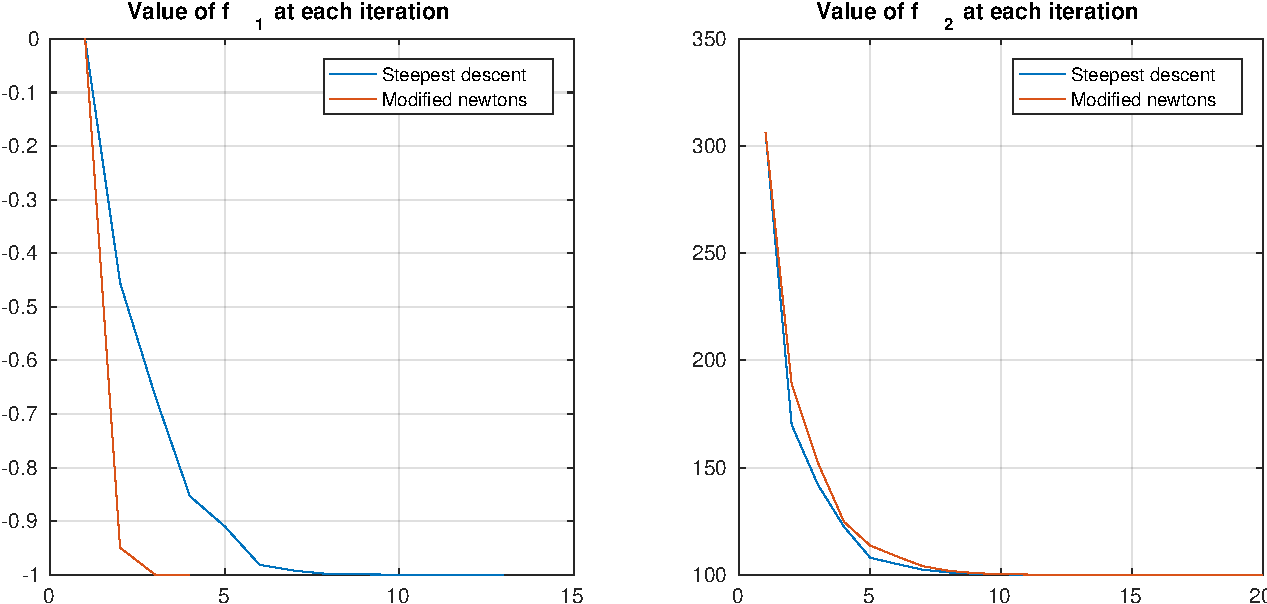
\includegraphics[width=\linewidth]{fig/unconstrained_exercices/pb7_1-crop}


\textbf{g)}

\answer

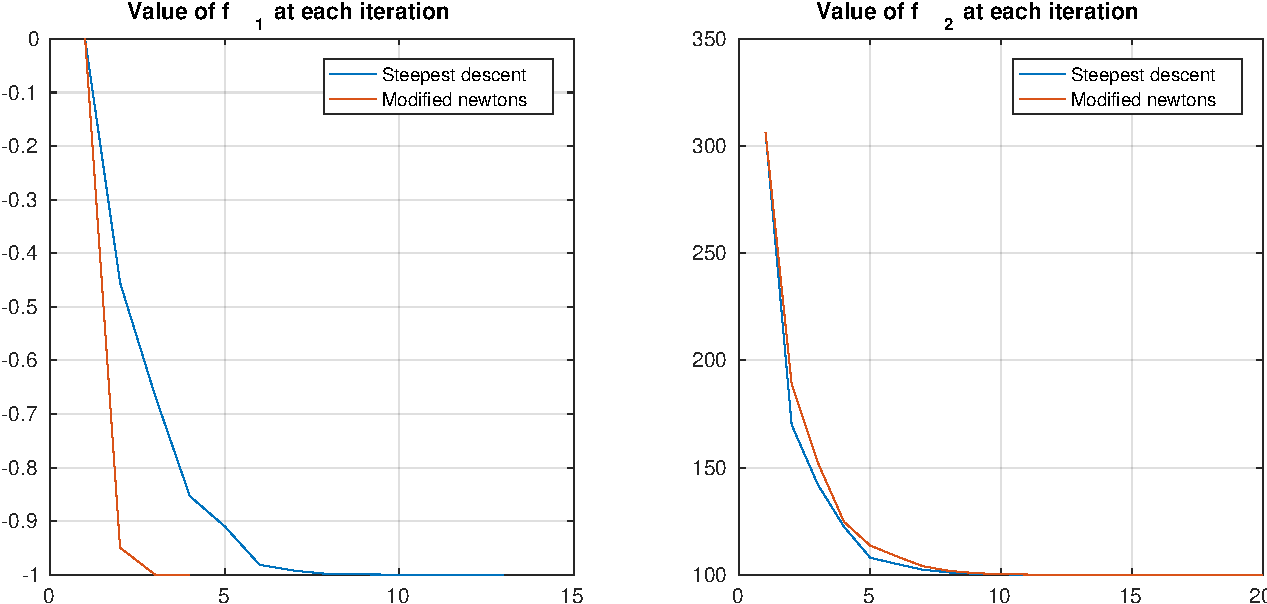
\includegraphics[width=\linewidth]{fig/unconstrained_exercices/pb7_1-crop}


\subsection{Problem 8}

\textbf{a)}

On school desktop

\textbf{b)}

On school desktop, SR1

\textbf{c)}

Too long, the algebra didn't work :( ...

\subsection{Problem 9}

